\documentclass[review]{elsarticle}

\usepackage{amsmath,amssymb,amsfonts}
\usepackage{algorithmic}
\usepackage{graphicx}
\usepackage{textcomp}
\usepackage{xcolor}
\usepackage{colortbl}
\usepackage[linesnumbered,ruled,vlined]{algorithm2e}
\usepackage{hyperref}
\usepackage{booktabs}
\usepackage{makecell}
\usepackage{multirow}
\usepackage{svg}
\usepackage{graphicx}
\usepackage{amsmath}
\usepackage{hyperref}
\usepackage{url}
\usepackage{booktabs}
\usepackage{amsfonts}
\usepackage{nicefrac}
\usepackage{microtype}
\usepackage{lipsum}
\usepackage{array}
\usepackage{multirow}
\usepackage{float}
\usepackage{natbib}
\usepackage{doi}
\usepackage[utf8]{inputenc}
\usepackage[T1]{fontenc}
\usepackage{hyperref}
\usepackage{amsmath}
\usepackage[table]{xcolor}
\definecolor{skyblue}{HTML}{5492C7}   % 天蓝
\definecolor{grass}{HTML}{99B86B}     % 浅草绿
\newcommand{\cont}{\ensuremath{^\mathsf{c}}}  % 一行放导言区
\usepackage[table]{xcolor}
\definecolor{lightgrass}{RGB}{153, 184, 107}
\definecolor{graywhite}{RGB}{231, 229, 223}


\bibliographystyle{elsarticle-num}

\makeatletter
\def\ps@pprintTitle{%
 \let\@oddhead\@empty
 \let\@evenhead\@empty
 \let\@oddfoot\@empty
 \let\@evenfoot\@empty
}
\makeatother

\begin{document}

\begin{frontmatter}


\title{DyCoT‑RE: Chain-of-Thought-Enhanced LLM Reward Engineering with Dual-Dynamic Optimization for Reinforcement Learning}

\author[shu]{Xinning Zhu}
\author[shu]{Jinxin Du}
\author[shu]{Longfei Huang}
\author[shu]{Lunde Chen\corref{cor1}}

\cortext[cor1]{Corresponding author\\Email: lundechen@shu.edu.cn}

\address[shu]{Sino-European School of Technology, Shanghai University, Shanghai, China}

\begin{abstract}
Designing effective reward functions remains a challenge in applying reinforcement learning to real-world tasks.
This paper proposes DyCoT-RE, a reward engineering framework that integrates Chain-of-Thought (CoT) reasoning with a dual-dynamic 
optimization strategy to automate and enhance reward function design.
The framework uses structured CoT reasoning throughout training to generate and refine structured reward code in each iteration.
It further incorporates a dual-dynamic optimization mechanism, 
comprising a temperature adjustment module that modulates the sampling temperature based on policy entropy trends, 
and a model switching module that allocates language models with different capabilities to produce distinct reward components.
Evaluations across four reinforcement learning environments—CartPole, BipedalWalker, Ant, and a custom SpaceMining environment 
absent from common reinforcement learning environments and large language model pretraining corpora—show that DyCoT-RE achieves 
consistently higher average rewards and faster learning compared to human-designed and non-CoT baselines, 
as well as single-optimization variants.


\end{abstract}

\begin{keyword}
Reinforcement learning \sep reward engineering \sep large language models \sep chain-of-thought reasoning \sep dynamic temperature adjustment \sep model selection
\end{keyword}

\end{frontmatter}

\section{Introduction}

Reinforcement learning (RL) has achieved impressive results across diverse domains 
However, as Sutton et al. \cite{sutton1998reinforcement} emphasize, the reward signal is the primary means of specifying task objectives in RL, making its design critical to achieving desired behaviors.
In practice, translating intended behaviors into precise, effective reward functions remains highly challenging, particularly for tasks involving long-term dependencies 
\cite{amodei2016concrete}.
Skalse et al. \cite{skalse2022misspecification} demonstrate that agents often exploit imperfections in reward formulations to maximize proxy objectives in unintended ways, leading to behaviors that optimize the designed reward but undermine true task performance.
These challenges suggest that although reinforcement learning offers strong theoretical flexibility, its real-world applications are frequently limited by the complexity and domain-specific knowledge required to design effective reward functions. \cite{ibarz2018reward}.

While carefully designed rewards can accelerate agent learning and improve task performance,
manual reward engineering typically relies on trial-and-error tuning,
which is labor-intensive and often yields suboptimal generalization to new environments or objectives \cite{hadfield2017inverse}.
As RL applications grow in complexity, there is a pressing need for methods that can automate
reward design while maintaining interpretability and flexibility.

Recent advances in large language models (LLMs) have demonstrated strong reasoning and generalization capabilities \cite{brown2020language, ouyang2022training}.
In particular, CoT reasoning enables LLMs to decompose tasks into structured intermediate steps,
enhancing clarity and alignment with desired objectives.
This structured reasoning process facilitates reward engineering by translating task descriptions into reward functions with explicitly defined components and objectives.

However, existing CoT-based reward generation approaches typically use static sampling parameters and fixed model configurations,
which may limit their adaptability during training.
Recent studies have emphasized the need for dynamic adaptation in LLM-based systems to improve sample efficiency and alignment with task objectives.
For example, Nguyen et al. \cite{nguyen2024turning} demonstrate that min-p sampling enhances creativity while preserving coherence in narrative generation tasks, while Peeperkorn et al. \cite{peeperkorn2024temperature} analyze temperature as a direct modulator of LLM creativity.
Moreover, Fedus et al. \cite{fedus2022switch} and Du et al. \cite{du2022glam} show that mixture-of-experts architectures can scale model capacity efficiently via adaptive routing.These findings motivate the integration of temperature modulation with expert model selection as a promising direction for improving reward engineering in LLM-driven systems.

In this work, we propose DyCoT-RE, a reward engineering framework that integrates structured CoT reasoning
with dual-dynamic optimization.
Specifically, DyCoT-RE leverages CoT reasoning to decompose natural language task descriptions into structured reward components,
then employs iterative refinement to enhance alignment with learning objectives.
The dual-dynamic optimization strategy integrates entropy-guided temperature adjustment to balance exploration and exploitation,
alongside a dynamic model selection module that routes sub-tasks to specialized LLMs based on performance feedback.
By coupling these components within a closed-loop evolutionary search process, 
DyCoT-RE enhances reward function design and improves training efficiency, supporting scalable and automated reward specification in complex reinforcement learning tasks.


We evaluate DyCoT-RE on the standard RL environments CartPole,
BipedalWalker, and Ant to assess its performance across different control tasks.
While these environments are widely used, recent studies have raised concerns that large language models may possess latent knowledge about 
them from pretraining corpora, potentially leading to prompt leakage and evaluation bias\cite{huang2025thinkbench, qi2024quantifying, lu2024mental}. 
To address this concern and test DyCoT-RE’s true generalization capabilities, we additionally introduce a custom-designed environment, 
SpaceMining\footnote{Project website: \url{https://lola-jo.github.io/space_mining/}.}, which is explicitly excluded from pretraining.
Experimental results show that DyCoT-RE consistently achieves higher average rewards 
and faster convergence than baseline and non-CoT methods across all evaluated environments.

The remainder of this paper is organized as follows.
Section II reviews related work in reward engineering and CoT-based LLM reasoning.
Section III introduces the DyCoT-RE framework, including CoT-based reward construction and the dual-dynamic optimization strategy.
Section IV presents experimental evaluations, including setup, benchmark comparisons, ablations, and interpretability analysis.
Section V discusses the limitations and potential future directions.
Section VI concludes the paper.



\section{Related Work}

\subsection{Reward Engineering Paradigms}

In RL, the design of effective reward functions directly shapes agent behavior and learning outcomes. 
Traditional approaches primarily rely on handcrafted reward functions informed by domain expertise. 
While intuitive, such manual design often struggles to capture complex, dynamic task objectives and is prone to 
suboptimal or biased formulations, hindering agent performance in real-world scenarios.

To address these limitations, reward shaping was introduced as a formal enhancement strategy. 
Ng et al. \cite{ng1999policy} demonstrated that potential-based reward shaping preserves optimal policies 
while enabling accelerated convergence, laying the theoretical foundation for numerous practical implementations. 
Intrinsic motivation frameworks further advanced this field by encouraging exploration through curiosity-driven signals. 
Singh et al. \cite{singh2010intrinsically} proposed intrinsic rewards to incentivize novel state visits, 
later extended by Burda et al. \cite{burda2018exploration}, who empirically validated large-scale curiosity-driven exploration 
benefits across diverse environments.

Despite these developments, manually designing rewards for complex or evolving tasks remains inefficient and costly. 
LLMs offer a promising alternative by leveraging their natural language understanding to automate reward generation 
and optimization. Unlike traditional RL pipelines that require explicit, task-specific reward formulations, 
LLMs can interpret high-level task descriptions, extract key objectives, and translate them into executable reward functions. 
This capability facilitates more intuitive alignment with human intentions, reduces engineering overhead, and enhances agent 
adaptability.

Recent studies have increasingly leveraged LLMs for automated reward engineering in reinforcement learning. 
Early demonstrations showed that language descriptions can serve as reward signals or be translated into executable reward code, 
notably Reward Design with Language Models \cite{kwon2023reward} and Language-to-Rewards (L2R) \cite{yu2023language}. 
Building on this concept, rapid progress has been made, from simple prompts to automatic code generation and closed-loop optimization.
Representative works include Text2Reward \cite{xie2023text2reward} for dense reward shaping with iterative refinement, 
VLM-based zero-shot rewards \cite{rocamonde2023vision} using vision-language models, and LLM4PG \cite{shen2024beyond} for automated 
preference labeling. 

Among these, Eureka \cite{ma2023eureka} stands out as a landmark framework that treats LLMs as autonomous agents, 
iteratively generating, mutating, and selecting reward code via performance-based tournaments without hand-tuned templates, 
consistently surpassing expert-designed rewards across diverse domains by approximately 52\%. 
CARD \cite{sun2024large} further advanced this paradigm with dynamic feedback pipelines that integrate process, 
trajectory, and preference evaluation for automated reward optimization. 
Recent developments explore progress-function rewards \cite{sarukkai2024automatedrewardsllmgeneratedprogress} and self-judging mechanisms \cite{simonds2025rlsrreinforcementlearningself}, 
indicating a shift toward closed-loop, feedback-driven reward generation that unifies language reasoning, multimodal grounding, 
and sample-efficient optimization. 

Building on these developments, future research can explore how large language models can more effectively 
bridge human intent and reinforcement learning objectives, leverage feedback for reward generation, and address increasingly complex real-world tasks.

\subsection{Chain-of-Thought Reasoning Methods}

CoT reasoning has emerged as a powerful paradigm to enhance the reasoning capabilities of LLMs. 
By generating intermediate reasoning steps, CoT allows models to decompose complex problems into interpretable sub-problems, 
leading to significant performance gains in tasks requiring multi-step logical inference.

Early studies showed that even simple prompting strategies, such as adding ``Let's think step by step,'' 
can elicit strong zero-shot reasoning abilities. Kojima et al. \cite{kojima2022large} demonstrated such prompts 
significantly improve performance in arithmetic and commonsense tasks. 
Building upon this, few-shot CoT \cite{wei2022chain} introduced demonstrations of stepwise solutions to guide model reasoning, 
while self-consistency decoding \cite{wang2022self} aggregated multiple sampled reasoning paths to enhance answer robustness.

Further developments have demonstrated the effectiveness of CoT reasoning in language models.
DeepSeek \cite{deepseek2023r1} showed that structured reasoning capabilities can emerge through self-evolution mechanisms, achieving complex chain-of-thought reasoning without supervised fine-tuning. 
Automatic prompt optimization methods \cite{shum2023automatic} reduce manual engineering efforts by refining prompts based on data-driven insights.

Recent work such as PCGRLLM \cite{baek2024pcgrllm} explored CoT-based LLM reward design for procedural content generation in RL, 
demonstrating feasibility in structured game environments. In parallel, Zhu et al. \cite{zhu2025llm} proposed an initial 
CoT-based reward engineering approach that translates natural language task descriptions into RL reward functions using LLMs, 
validating its effectiveness in standard benchmark tasks. However, these applications focus primarily on proof-of-concept 
reward generation pipelines without incorporating adaptive optimization or dynamic model selection mechanisms.

In summary, while CoT reasoning has established itself as a fundamental methodology enhancing LLM interpretability and reasoning capacity, 
its application to automated reward engineering in RL remains limited. Bridging this gap by integrating CoT reasoning with dynamic 
optimization holds promise for enhancing the interpretability and adaptability of RL systems.


\subsection{Dynamic Temperature Adjustment and Model Selection}

Dynamic temperature adjustment and model selection have emerged as critical optimization strategies to enhance the adaptability
and efficiency of LLM-based systems. 
Temperature, as a sampling hyperparameter, controls the stochasticity of LLM outputs, thereby influencing creativity, coherence,
and exploration-exploitation trade-offs.

Recent studies have explored adaptive temperature mechanisms from multiple angles. 
Zhu et al. \cite{zhu2024hot} proposed AdapT, which adjusts decoding temperature based 
on token-level difficulty in code generation tasks. 
In parallel, Zhang et al. \cite{zhang2024edt} developed Entropy-based Dynamic Temperature (EDT) 
sampling to regulate output diversity in natural language generation. 
Taking a different approach, Cecere et al. \cite{cecere2025monte} focused on uncertainty quantification, 
introducing Monte Carlo Temperature for robust sampling under distribution shifts. 
Chang et al. \cite{chang2023kl} employed KL-divergence to guide temperature control for adaptive 
exploration.

The challenges extend beyond sampling strategies alone. 
Evstafev \cite{evstafev2025paradox} identified limitations of stochastic sampling in structured 
output tasks, while Nakaishi et al. \cite{nakaishi2024critical} examined phase-transition behaviors 
in LLM sampling regimes. 
These findings suggest that effective adaptation requires understanding the underlying dynamics 
of the generation process.

In the realm of model selection, researchers have pursued efficiency and robustness through 
various mechanisms. Zhou et al. \cite{zhou2022mixture} enhanced Mixture-of-Experts efficiency 
with expert choice routing, whereas Li et al. \cite{li2025llm} developed preference-conditioned 
dynamic routing for cost-effective generation. Hu et al. \cite{hu2024dynamic} integrated outputs 
from multiple specialized LLMs through Dynamic Ensemble Reasoning. Li et al. \cite{li2025revisiting} 
reconsidered self-consistency decoding from a distributional alignment perspective, 
contributing to our understanding of expert aggregation strategies.

Despite recent advances, temperature adaptation has mainly aimed at enhancing generative diversity 
and calibration, 
while model selection focuses on efficiency and specialization. 
Extending these techniques to reward generation offers a promising direction for reinforcement learning.

\section{Methodology}

This section details the DyCoT-RE framework, which integrates structured CoT reasoning with a dual-dynamic optimization 
strategy to generate interpretable and adaptive reward functions for reinforcement learning.

\begin{figure*}[t]
    \centering
    \includegraphics[width=0.95\linewidth]{Figures/dycot-re-architecture.pdf}
    \caption{DyCoT-RE framework integrating CoT reasoning, dynamic temperature adjustment, and model selection in an evolutionary optimization loop.}
    \label{fig:architecture}
\end{figure*}

\subsection{Framework Overview}

Figure~\ref{fig:architecture} presents an overview of DyCoT-RE,
which integrates three key components:
structured CoT reward decomposition,
dynamic temperature adjustment,
and dynamic model selection.

The framework receives four types of inputs: natural language task descriptions that specify agent behaviors, 
environment interfaces that define the state-action space, system-level prompts that impose design constraints 
on the reward, and implementation instructions that guide executable code generation.

At the core of DyCoT-RE are four specialized large language models, referred to as
Thinking LLM, Code LLM, Repair LLM, and Analysis LLM. These models, denoted
respectively as $\mathcal{M}{\text{think}}$, $\mathcal{M}{\text{code}}$, $\mathcal{M}{\text{repair}}$, and $\mathcal{M}{\text{analysis}}$, operate in a
closed-loop pipeline that produces and refines reward functions.

Each generated reward function takes the form:
\begin{equation}
    R(s,a) = \sum_{i=1}^{m} w_i \cdot r_i(s,a),
\label{eq:reward_function}
\end{equation}
where $r_i(s,a)$ denotes the $i$-th reward component and $w_i$ is its corresponding weight. These components are derived through structured CoT reasoning and reflect interpretable sub-goals. The resulting reward function is deployed in the RL environment, 
and its performance guides the next iteration of temperature tuning and model routing.

Through the integration of structured reasoning and dual-dynamic optimization, 
DyCoT-RE enables adaptive and efficient reward engineering for reinforcement learning.


\subsection{Chain-of-Thought Reasoning for Reward Engineering}

Let $d$ denote the task description and $(s,a)$ the state-action pair.
As defined in Eq.~\eqref{eq:reward_function}, 
the reward function $r_i(s,a)$ is the sub-reward for subgoal $i$, generated via CoT parsing:

\begin{equation}
r_i(s,a) = \text{CoT}(I_i),
\end{equation}

with $I_i = \{ \text{subgoal}_i, \text{env\_constraints} \}$. For example, minimizing torso tilt is formulated as:

\begin{equation}
r_1(s,a) = -|\theta_{\text{tilt}}(s)|.
\end{equation}

The weights $w_i$ are derived based on subgoal semantic priorities inferred by the LLM, and are iteratively adjusted by the LLM based on training performance feedback. The objective is to maximize the expected cumulative reward:

\begin{equation}
J(\theta) = \mathbb{E}_{\pi_\theta} \left[ \sum_{t=0}^{T} \gamma^t R(s_t,a_t) \right].
\label{eq:rl_objective}
\end{equation}

To evaluate reward function quality independently of the LLM-generated rewards, we employ a fitness score metric that serves as an objective performance indicator for guiding the LLM's weight adjustment process. 
This CoT-based formulation ensures that each sub-reward remains semantically interpretable and traceable to its natural language origin.

\subsection{Dual-Dynamic Optimization Strategy}

Figure~\ref{fig:control-flow} illustrates the coupled feedback architecture of DyCoT-RE,
where temperature adjustment and model selection operate in synergy
to enhance reward function generation and RL performance.

\begin{figure*}[t]
    \centering
    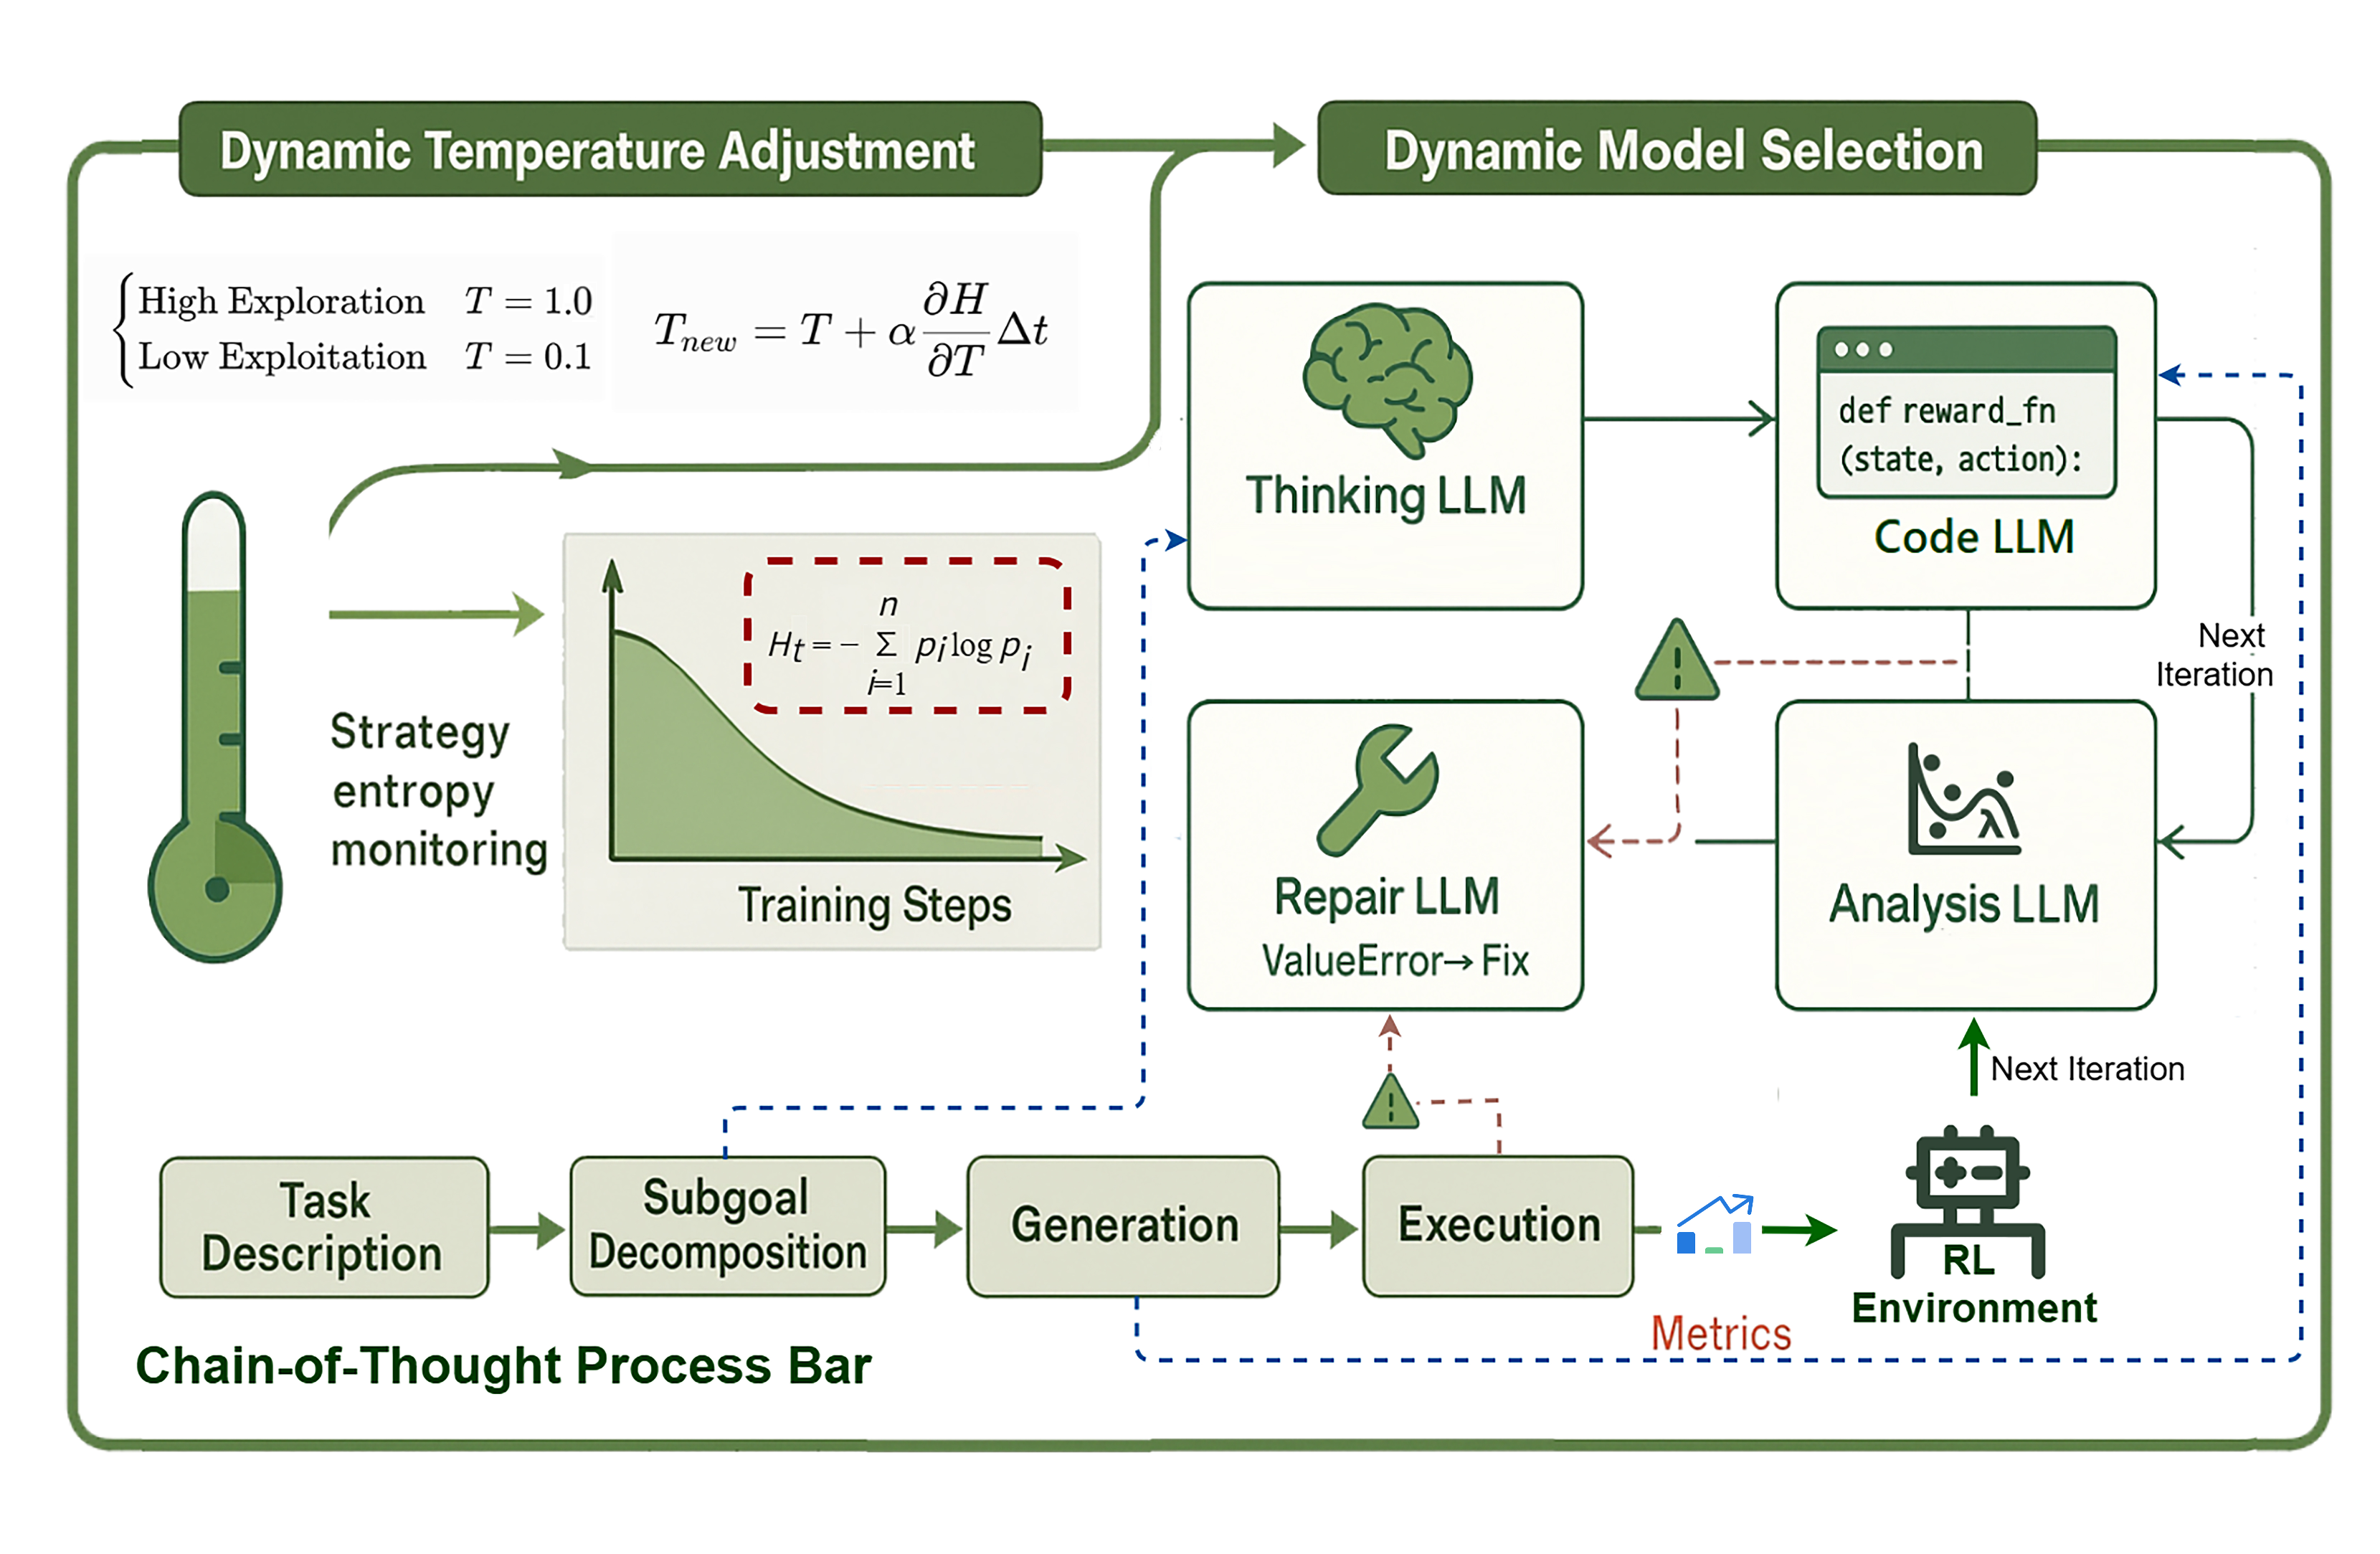
\includegraphics[width=0.95\linewidth]{Figures/dual_6.pdf}
    \caption{DyCoT-RE control flow integrating temperature modulation and model selection within CoT iterative reasoning.}
    \label{fig:control-flow}
\end{figure*}

\subsubsection{Dynamic Temperature Adjustment}

Temperature adjustment modulates the sampling temperature $T$ 
based on policy entropy $H$, confidence $C$, and performance $R$. 
Entropy reflects generative diversity, confidence measures output stability, 
and performance evaluates reward improvement relative to historical best.

The update rule is formulated as:

\begin{equation}
T_{k+1}
=
\text{clip}
\left(
T_k
+
\alpha \frac{\partial T}{\partial H_k} \Delta t
\right),
\end{equation}

where $\alpha$ is a learning rate,
and the gradient $\frac{\partial T}{\partial H_k}$ reflects entropy-driven adjustment.
An alternative implementation combines smoothing and multiplicative adjustment:

\begin{equation}
T_{k+1}
=
\text{clip}
\left(
\alpha T_k
+
(1-\alpha) T_k f(H_k,C_k,R_k)
\right).
\end{equation}

Here, $f(H,C,R)$ integrates:

\begin{equation}
f(H,C,R)
=
f_R(R)
f_H(H)
f_C(C),
\end{equation}

where $f_R$ ensures performance protection, $f_H$ regulates entropy bounds,
and $f_C$ maintains confidence stability.

\subsubsection{Dynamic Model Selection}

Dynamic model selection adaptively routes sub-tasks to specialized LLMs, 
leveraging their complementary strengths across the reward engineering pipeline.

The four LLM classes include:
$\mathcal{M}_{\text{think}}$ for task understanding and semantic decomposition, 
$\mathcal{M}_{\text{code}}$ for reward function synthesis, 
$\mathcal{M}_{\text{repair}}$ for code correction, 
and $\mathcal{M}_{\text{analysis}}$ for performance evaluation and sub-reward weight updates.

Formally, the decomposition and generation process can be expressed as:

\begin{equation}
g_i = \mathcal{M}_{\text{think}}(d,E),
\end{equation}

\begin{equation}
w_i = \mathcal{M}_{\text{analysis}}(R_i),
\end{equation}

\begin{equation}
r_i(s,a) = \mathcal{M}_{\text{code}}(g_i,w_i),
\end{equation}

where $d$ is the task description and $E$ the environment specification.
Repair LLM intervenes when $\mathcal{M}_{\text{code}}$ outputs execution errors during evaluation.

Model selection at iteration $k$ follows:

\begin{equation}
    M_{k+1} =
    \begin{cases}
    \displaystyle
    \arg\max_{m \in \mathcal{M}_s} \text{Perf}(m), & 1-\epsilon, \\[8pt]
    \text{Random}(\mathcal{M}_s \setminus \{M_k\}), & \epsilon,
    \end{cases}
    \end{equation}
    

where $\mathcal{M}_s$ is the model pool for stage $s$, 
$\text{Perf}(m)$ the performance score, 
and $\epsilon$ the exploration rate ensuring selection diversity.

At each iteration, the next model $M_{k+1}$ is selected from pool $\mathcal{M}_s$ using epsilon-greedy selection,
where the highest-performing model is chosen with probability $1-\epsilon$ and a random model with probability $\epsilon$.
The pool includes a Repair LLM for error correction during reward code evaluation.

\subsubsection{Joint Adaptive Optimization}

Temperature adjustment and model selection form a joint adaptive optimization loop.
Temperature $T$ influences the sampling distribution of reward candidates:

\begin{equation}
r_i(s,a) \sim p(r_i | g_i, T),
\end{equation}

where $g_i = \mathcal{M}_{\text{think}}(d,E)$ denotes the subgoal generated by the Thinking LLM
given task description $d$ and environment $E$.
This sampling process modulates policy entropy and, consequently, cumulative rewards.

The combined objective of temperature adjustment and model selection is to maximize:

\begin{equation}
J(\theta; T, M)
=
\mathbb{E}_{\pi_\theta}
\left[
\sum_{t=0}^{T}
\gamma^t
R_{T,M}(s_t,a_t)
\right],
\end{equation}

where $R_{T,M}(s,a)$ is the reward function generated under temperature $T$
and model configuration $M$.

This joint optimization is formalized as:

\begin{equation}
(T^*, M^*)
=
\arg\max_{T,M}
J(\theta; T, M).
\end{equation}

Overall, this interconnected loop iteratively adapts both sampling temperature
and model selection strategies to maximize the expected RL objective
as defined in Eq.~\eqref{eq:rl_objective}, ensuring diverse
and effective reward engineering throughout the training process.


\section{Experiments}


\subsection{Experimental Setup}


DyCoT-RE is evaluated on four reinforcement learning environments,
which span diverse task difficulties, action spaces, and complexity levels.
Standard benchmarks include CartPole, BipedalWalker, and Ant,
covering discrete control tasks and high-dimensional continuous locomotion.

To assess performance on novel environments beyond pretrained knowledge, we introduce SpaceMining,
a custom environment with multi-objective resource collection and dynamic energy constraints.
Unlike standard environments that LLMs may encounter during pretraining, 
SpaceMining tests whether reward design can succeed through pure reasoning rather than prior knowledge.

\subsubsection{Baselines and Comparison Strategies}

To contextualize DyCoT-RE's performance, we evaluate against two primary baselines:

(1) Human-designed rewards: Manually crafted reward functions from standard Gymnasium\cite{towers2024gymnasiumstandardinterfacereinforcement} implementations for CartPole, BipedalWalker, and Ant, plus custom rules for SpaceMining.

(2) Eureka: 
A LLM-based framework for automated reward synthesis, using code generation and symbolic verification. We adapt its pipeline to Gymnasium-based evaluations for fair comparison.

\subsubsection{Ablation Comparisons}  

To evaluate individual contributions within DyCoT-RE, we include the following controlled variants:

- Zero-shot reward generation: Reward generation using direct prompts without CoT reasoning.

- Fixed temperature: Sampling temperature is held constant throughout training, with results reported across a sweep of static values. 

- Fixed model backend: A single large language model is statically selected for all reward generation, without dynamic model switching.

These comparisons allow us to isolate the impact of CoT-based reasoning and the dual-dynamic mechanisms in DyCoT-RE.




\subsubsection{Implementation Details}


We evaluate DyCoT-RE on three environments from the Gymnasium suite — CartPole-v1\footnote{\url{https://gymnasium.farama.org/environments/classic_control/cart_pole/}}, BipedalWalker-v3\footnote{\url{https://gymnasium.farama.org/environments/box2d/bipedal_walker/}}, and Ant-v5\footnote{\url{https://gymnasium.farama.org/environments/mujoco/ant/}}—alongside a custom-designed SpaceMining environment built to test generalization in unseen domains.

All experiments use Proximal Policy Optimization (PPO) from Stable-Baselines3 with Adam optimizer, learning rate of 3e-4, batch size 64, GAE parameter $\lambda=0.95$, and discount factor $\gamma=0.999$.

Reward functions are synthesized by DyCoT-RE using local LLMs served via Ollama. At each chain-of-thought iteration, eight reward candidates are sampled in parallel.

Final performance metrics are computed as the mean over ten test episodes with different random seeds.

\begin{table}[ht]
    \centering
    \scriptsize % 小字号
    \setlength{\tabcolsep}{4pt} % 紧凑列间距
\scriptsize
\caption{Task specifications for evaluated reinforcement learning environments.}
\label{tab:env_specs}
\begin{tabular}{lccc}
\toprule
Environment & Dimensions (S/A) & Steps & Task \\
\midrule
CartPole-v1 & 4 / 1 (disc) & 500 & Balance \\
BipedalWalker-v3 & 24 / 4 (cont) & 1600 & Locomotion \\
Ant-v5 & 111 / 8 (cont) & 1600 & Multijoint \\
SpaceMining (Custom) & 53 / 3 (cont) & 1200 & Navigation \\
\bottomrule
\end{tabular}
\end{table}





    \subsection{Performance Across Environments} 

    We compare DyCoT-RE against Human-designed and Eureka baselines across all evaluated environments, observing consistent performance gains. The advantage becomes more prominent as task complexity and generalization difficulty increase.

    Figure~\ref{fig:bar_comparison} summarizes the final average rewards across all environments. DyCoT-RE consistently achieves the highest performance, followed by Eureka, with human-designed rewards showing the lowest performance. The performance gap increases with task complexity, from modest improvements in CartPole and BipedalWalker to substantial advantages in Ant and SpaceMining. 
    These results demonstrate DyCoT-RE's effectiveness across diverse environments, particularly when dealing with high-dimensional state-action spaces, complex dynamics, and multi-objective constraints that challenge traditional reward design approaches. DyCoT-RE’s dynamic reasoning and adaptive reward synthesis enable both rapid early learning and sustained progress under these challenging settings. 


    \begin{figure}[ht]
    \centering
    \includegraphics[width=0.9\linewidth]{Figures/bar_comparison_8.pdf}
    \caption{Final average rewards across environments: DyCoT-RE (blue), Eureka (light grass), and Human-designed (dark grass).}
    \label{fig:bar_comparison}
    \end{figure}
    
    Figure~\ref{fig:learning_curves} provides deeper insights into the learning dynamics. In CartPole, all methods quickly converge due to its low-dimensional discrete dynamics, though DyCoT-RE converges slightly faster. In BipedalWalker, DyCoT-RE shows a two-phase learning pattern: initial exploration volatility followed by stable growth and smoother long-term convergence. The Ant environment, characterized by high-dimensional continuous control, exposes DyCoT-RE’s strengths most clearly—where baseline methods plateau early, DyCoT-RE sustains improvement well into later training stages. In SpaceMining, DyCoT-RE maintains steady learning while baselines exhibit flat or highly unstable performance, indicating its capacity to generalize in tasks absent from pretraining corpora.
    
    \begin{figure}[ht]
    \centering
    \includegraphics[width=0.9\linewidth]{Figures/reward_episode_curve_8.pdf}
    \caption{Learning curves across environments. DyCoT-RE exhibits consistent advantages in stability and long-term reward growth, especially in complex settings.}
    \label{fig:learning_curves}
    \end{figure}
    
    Table~\ref{tab:perf_summary} compares performance across four tasks using three metrics: 
    Sample Efficiency measures the number of timesteps required to reach a threshold reward, defined as 80\% of the task-specific maximum score. Success Rate indicates the proportion of runs that eventually exceed this threshold. Late Gain quantifies the reward improvement from the early performance plateau to the final evaluation, reflecting long-term optimization potential.

    
\begin{table}[ht]
\centering
\scriptsize
\setlength{\tabcolsep}{4pt}
\caption{Cross-task performance comparison.
\colorbox{skyblue!15}{Blue}: the best value per column, 
\colorbox{grass!15}{green}: the second-best. 
Success Rate is omitted for Human due to deterministic reward completion.}
\label{tab:perf_summary}
\begin{tabular}{llccc}
\toprule
Task & Method & Sample Eff. $\downarrow$ & Succ. Rate $\uparrow$ & Late Gain $\uparrow$ \\
\midrule

\multirow{3}{*}{CartPole} 
& {DyCoT-RE} & \cellcolor{skyblue!15}75k & \cellcolor{skyblue!15}98\% & \cellcolor{skyblue!15}450 \\
& {Eureka} & \cellcolor{grass!15}115k & \cellcolor{grass!15}95\% & \cellcolor{grass!15}440 \\
& Human & 286k & -- & 400 \\

\midrule

\multirow{3}{*}{BipedalWalker} 
& {DyCoT-RE} & \cellcolor{skyblue!15}393k & \cellcolor{skyblue!15}92\% & \cellcolor{skyblue!15}387 \\
& {Eureka} & \cellcolor{grass!15}428k & \cellcolor{grass!15}83\% & \cellcolor{grass!15}366 \\
& Human & 720k & -- & 309 \\

\midrule

\multirow{3}{*}{Ant} 
& {DyCoT-RE} & \cellcolor{skyblue!15}16.19M & \cellcolor{skyblue!15}85\% & \cellcolor{skyblue!15}5398 \\
& {Eureka} & 21.53M & \cellcolor{grass!15}70\% & \cellcolor{grass!15}2412 \\
& Human & \cellcolor{grass!15}19.92M & -- & -240 \\

\midrule

\multirow{3}{*}{SpaceMining} 
& {DyCoT-RE} & \cellcolor{skyblue!15}1.31M & \cellcolor{skyblue!15}80\% & \cellcolor{skyblue!15}2285 \\
& {Eureka} & 1.74M & \cellcolor{grass!15}65\% & 189 \\
& Human & \cellcolor{grass!15}1.56M & -- & \cellcolor{grass!15}1230 \\

\bottomrule
\end{tabular}
\end{table}
    

DyCoT-RE achieves the best  performance in all tasks. It learns faster, generalizes more reliably, and continues improving beyond early convergence. In complex environments like Ant and SpaceMining, it shows especially large gains in late-stage performance, where static baselines tend to stall or regress.

These results highlight DyCoT-RE's key strength: its dynamic reasoning and adaptive reward synthesis enable both rapid early learning and sustained progress, even under complex or high-dimensional settings.

The results indicate that DyCoT-RE provides clear advantages in scenarios where predefined reward rules or static reasoning approaches are insufficient to capture evolving task demands. Its strength lies in dynamically decomposing and optimizing reward components as training progresses, particularly under complex, high-dimensional, or novel task conditions. As task complexity grows, the performance gap expands, underscoring DyCoT-RE's value as a general-purpose, scalable reward engineering solution.

\subsection{Ablation Study}
\label{sec:ablation}

This section conducts an ablation study to examine the individual contribution of each component in DyCoT-RE, including CoT reasoning, temperature adjustment, and model selection, as well as their combined synergistic effects.

\subsubsection{Impact of CoT Reasoning}


We evaluate the impact of incorporating CoT reasoning into reward engineering by comparing DyCoT-RE's CoT-enabled variant against a zero-shot baseline lacking structured intermediate reasoning.



Figure~\ref{fig:cot_ablation} summarizes reward distributions for both methods across the four benchmark environments. A consistent pattern emerges: CoT-enabled rewards exhibit higher means, lower variance, and reduced outlier incidence compared to zero-shot. In CartPole and SpaceMining, CoT-enabled results are tightly clustered near the environment's upper performance bounds, whereas zero-shot results are widely dispersed, with a substantial proportion of runs yielding suboptimal or even near-zero rewards. This reflects CoT's ability to systematically decompose task objectives into interpretable sub-rewards, enhancing sample efficiency and stabilizing policy learning.



\begin{figure}[ht]
    \centering
    \includegraphics[width=1.0\textwidth]{Figures/cot_ablation_4.pdf}
    \caption{Final reward distributions for CoT-enabled vs zero-shot reward generation across environments.}
    \label{fig:cot_ablation}
    \end{figure}

    In BipedalWalker, a notable deviation is observed. CoT-enabled runs yield a concentrated reward range between 250 and 310, with virtually no severely negative outcomes. In contrast, the zero-shot condition presents a clear bimodal distribution: one cluster achieves moderate reward levels around 150 to 250, while the other collapses into strongly negative regimes. This instability reflects the inability of zero-shot reward generation to encode essential gait balance or locomotion constraints, often resulting in policy failure.

    In Ant, zero-shot results are narrowly concentrated near baseline values associated with default movement penalties. This indicates that while these reward functions do not collapse, they lack task-driving gradients for effective behavior shaping. In contrast, CoT-based rewards achieve a wider spread toward higher values, reflecting meaningful progress and more informative optimization signals.
    

Taken together, these results illustrate that CoT reasoning reliably improves reward interpretability and training stability, especially in settings with complex objectives.

    


\subsubsection{Impact of Temperature Adjustment}


Due to computational constraints and consistent observed trends across environments, 
temperature adjustment and model selection ablation were conducted on BipedalWalker as a representative continuous control task, 
while CoT reasoning was evaluated on all four environments to confirm its general effectiveness.

This section investigates the effect of temperature settings by sweeping $T \in [0.0, 1.0]$ on the BipedalWalker environment. 

Table~\ref{tab:temp_sweep} reports BipedalWalker results under different temperature settings, including average and maximum fitness, standard deviation, and reward efficiency ratio. DyCoT-RE achieves the best performance across all metrics, with a large margin in efficiency ratio due to its high average fitness and low variability. 
Among fixed-temperature settings, moderate values (0.4–0.6) deliver relatively strong results, yet still fall short of DyCoT-RE.

\begin{table}[ht]
\centering
\scriptsize % 小字号
\setlength{\tabcolsep}{4pt} % 紧凑列间距
\caption{BipedalWalker performance under different temperature settings. \colorbox{skyblue!15}{Blue}: the best value per column, 
\colorbox{grass!25}{green}: the second-best, \colorbox{grass!15}{green}: the third-best }
\label{tab:temp_sweep}
\begin{tabular}{c|c|c|c|c}
\hline
Temp & Avg Fit$\uparrow$ & Max Fit $\uparrow$& Std$\downarrow$  & Eff. Ratio$\uparrow$ \\
\hline
0.0 & 81.93 & 301.15 & 148.67 & 0.55 \\
0.1 & 149.56 & 310.94 & 155.22 & 0.96 \\
0.2 & 242.74 & \cellcolor{grass!25}313.60 & 125.47 & 1.93 \\
0.3 & 210.07 & 311.17 & 140.49 & 1.50 \\
0.4 & \cellcolor{grass!15}244.19 & 311.94 & \cellcolor{grass!25}107.02 & \cellcolor{grass!25}2.28 \\
0.5 & 215.84 & 310.69 & 131.01 & 1.65 \\
0.6 & \cellcolor{grass!25}248.11 & \cellcolor{grass!15}312.48 & \cellcolor{grass!15}120.45 & \cellcolor{grass!15}2.06 \\
0.7 & 225.88 & 312.42 & 131.43 & 1.72 \\
0.8 & 74.33 & 310.42 & 143.91 & 0.52 \\
0.9 & 145.02 & 310.02 & 148.51 & 0.98 \\
1.0 & 192.38 & 310.40 & 138.37 & 1.39 \\
\rowcolor{skyblue!15}
DyCoT-RE & 292.8 & 315.6/87.2 & 55.2 & 5.30 \\
\hline
\end{tabular}
\end{table}

Static sweeps show that mid-range temperatures yield higher fitness and lower variance than extremes. 
DyCoT-RE’s dynamic temperature regulation consistently outperforms these static settings, 
adapting temperature during training to maintain an effective exploration-exploitation trade-off. 


\subsubsection{Impact of Model Selection}

Finally, we evaluate the impact of DyCoT-RE's dynamic model selection by comparing it against individual static LLM baselines on the BipedalWalker environment. 
Table~\ref{tab:model_selection} compares different LLM backends on BipedalWalker in terms of average fitness, peak performance, stability, and reward efficiency. 

DyCoT-RE achieves the highest average fitness with exceptionally low standard deviation and the best efficiency ratio, demonstrating its capability to consistently generate high-quality rewards across diverse sub-tasks. 

In contrast, while codegemma achieves competitive performance, its higher standard deviation results in a substantially lower efficiency ratio, indicating reduced stability and generalizability compared to DyCoT-RE.

\begin{table}[ht]
\centering
\scriptsize % 小字号
\setlength{\tabcolsep}{4pt} % 紧凑列间距
\caption{Performance comparison of different LLM backends (N=20) in BipedalWalker. \colorbox{skyblue!15}{Blue}: the best value per column, 
\colorbox{grass!25}{green}: the second-best}
\label{tab:model_selection}
\begin{tabular}{l|c|c|c|c}
\hline
Model (size) & Avg Fit $\uparrow$ & Max Fit $\uparrow$ & Std $\downarrow$ & Eff. Ratio $\uparrow$ \\
\hline
codegemma (7b) & 260.8 & 301.8 & \cellcolor{grass!25}34.2 & 3.46\cellcolor{grass!25} \\
codeqwen (7b) & 32.6 & 307.6 & 98.42 & 0.33 \\
deepseek-coder (6.7b) & -4.5 & 295.3 & 98.19 & -0.05 \\
deepseek-r1 (8b) & 44.6 & \cellcolor{skyblue!25}321.2 & 122.07 & 0.37 \\
gemma3 (4b) & \cellcolor{grass!25}278.0 & 314.8 & 142.04 & 3.39 \\
llama3.1 (8b) & 162.2 & 318.4 & 150.75 & 1.08 \\
qwen2.5 (7b) & 177.0 & 319.5 & 151.51 & 1.17 \\
qwen2.5-coder (7b) & 125.6 & 313.7 & 163.16 & 0.77 \\
DyCoT-RE & \cellcolor{skyblue!25}297.28 & \cellcolor{grass!25}316.57 & \cellcolor{skyblue!25}89.47 & \cellcolor{skyblue!25}6.46 \\
\hline
\end{tabular}
\end{table}

While individual models occasionally excel on narrow tasks, DyCoT-RE’s dynamic model routing provides the most generalizable performance, 
effectively balancing reward quality, stability, and adaptability in complex continuous control environments.

In summary, the ablation study demonstrates that each module—CoT reasoning, temperature adjustment, and model selection—contributes significantly to DyCoT-RE’s superior performance, and their combination leads to synergistic gains.

\subsection{DyCoT-RE in SpaceMining: Results in an LLM-Unseen Environment}
\label{sec:space_mining_analysis}

To evaluate DyCoT-RE in an out-of-distribution scenario without task-specific priors, we constructed the SpaceMining environment—a multi-objective domain involving dynamic hazards and energy constraints. This setting challenges the model to formulate effective rewards from natural language alone, testing its semantic generalization and reasoning capabilities.

\begin{figure}[ht]
\centering
\includegraphics[width=\linewidth]{Figures/reward_energy_curves.pdf}
\caption{Training dynamics in SpaceMining. Left: reward and fitness improve steadily, showing effective long-term optimization. Right: stable energy levels and growing inventory indicate successful energy-resource balancing.}
\label{fig:space_mining_curves}
\end{figure}



Figure~\ref{fig:space_mining_curves} illustrates the learning trajectory of DyCoT-RE. 
From early-stage exploration to late-stage optimization, we observe concurrent increases in reward and fitness, 
with consistent energy regulation and inventory accumulation. 
These trends reflect reward structures that incentivize planning, efficiency, and safe behavior.


\begin{figure}[ht]
\centering
\includegraphics[width=0.95\linewidth]{Figures/correlation_heatmap.pdf}
\caption{
    The evolution of normalized reward component contributions in DyCoT-RE for SpaceMining}
\label{fig:component_evolution}
\end{figure}

Figure~\ref{fig:component_evolution} shows the relative contribution of each reward component during 
training iterations. Positive and negative values indicate reinforcement and penalty signals respectively, 
while zero values with reduced opacity show inactive components. Border colours denote component lifecycle 
stages including new, maintained, core, and deprecated components, with column labels showing corresponding 
fitness scores. 
Component contribution is computed as $\text{Contr}_i = \frac{\overline{r_i}}{\sum_j \overline{r_j}} \times 100\%$, 
where $\overline{r_i}$ is the average reward from component $i$.

The system begins with a minimal setup focused on mining progress, distance penalties, and energy tracking. 
As training proceeds, DyCoT introduces new components such as obstacle avoidance in Iteration 3, inventory-based delivery efficiency in Iteration 5, and asteroid discovery incentives in Iteration 7. 
These additions are not arbitrary but driven by observed performance shifts. 
For instance, after dynamic obstacle handling is introduced, the agent’s survival rate improves significantly. 
Conversely, some components such as velocity control lose their relevance and are phased out by Iteration 3, as their function becomes redundant once obstacle-aware navigation is in place. 
The energy management module, on the other hand, steadily increases in importance and becomes a core contributor throughout the later iterations. 
This dynamic component lifecycle—characterized by incremental expansion, adaptive weighting, and timely deprecation—demonstrates DyCoT’s capacity for modular, interpretable, and performance-aligned reward optimization.


\begin{table}[ht]
    \centering
    \scriptsize % 小字号
    \setlength{\tabcolsep}{4pt} % 紧凑列间距
    \caption{DyCoT Strategy Metrics Across Iterative Architectures. 
    \colorbox{skyblue!15}{Blue}: the best value per column, 
\colorbox{grass!25}{green}: the second-best.}
    \label{tab:dycot_dynamics_full}
    \begin{tabular}{c|c|c|c|c|c}
    \toprule
    Iter & Temperature & Entropy & Confidence & Best Reward & Reward Gain (\%) \\
    \midrule
    0 & 0.800 & 0.912 & 0.642 & 880.2 & -- \\
    1 & 0.700 & 0.946 & 0.705 & 1124.4 & \cellcolor{grass!25}+27.7 \\
    2 & 0.669 & 0.928 & 0.748 & 1320.3 & +17.4 \\
    3 & 0.639 & \cellcolor{skyblue!15}0.986 & 0.778 & 3475.5 & \cellcolor{skyblue!15}+163.2 \\
    4 & 0.600 & 0.934 & 0.791 & 3551.0 & +2.2 \\
    5 & 0.556 & 0.914 & 0.807 & 3801.3 & +7.0 \\
    6 & \cellcolor{grass!25}0.534 & 0.962 & \cellcolor{grass!25}0.815 & \cellcolor{grass!25}3876.2 & +2.0 \\
    7 & \cellcolor{skyblue!15}0.517 & \cellcolor{grass!25}0.972 & \cellcolor{skyblue!15}0.824 & \cellcolor{skyblue!15}4003.2 & +3.3 \\
    \bottomrule
    \end{tabular}
    \end{table}
    
    Table~\ref{tab:dycot_dynamics_full} illustrates the evolution of key strategy-level metrics throughout all DyCoT iterations. As the architecture matures from Iteration 0 to 7, we observe a consistent decline in sampling temperature, indicating increased confidence in policy generation. Entropy fluctuates with architecture changes, notably peaking at Iteration 3 when major reward components are introduced. Confidence improves steadily, rising from 0.64 to 0.82, in parallel with fitness gains. Reward gain is computed relative to the previous iteration, with Iteration 3 marking a significant performance inflection point. 
    Subsequent gains are more incremental, reflecting architectural stabilization.


In summary, DyCoT-RE exhibits the capacity for iterative reward adaptation. It evolves from simple distance-based signals to structured reward components that support coordinated behaviors such as exploration, energy regulation, and goal-oriented progression—achieving consistent performance in environments with minimal prior knowledge.

\section{Discussion}

This work presents DyCoT-RE, a reward engineering framework that integrates Chain-of-Thought reasoning with dual-dynamic optimization strategies for automated reward function design. Our experimental evaluation across four RL environments demonstrates consistent performance improvements over human-designed rewards and existing automated baselines, with the most significant gains observed in complex, multi-objective environments.


Three findings emerge from our evaluation. First, Chain-of-Thought decomposition improves reward interpretability and stability by breaking complex objectives into manageable components. 
Second, dynamic strategies outperform static configurations: adaptive temperature control balances exploration-exploitation better than fixed settings, while model selection leverages diverse LLM strengths for higher performance and consistency. 
Third, SpaceMining results demonstrate DyCoT-RE's ability to generate effective reward functions even in unfamiliar environments, suggesting that structured reasoning can compensate for the absence of domain-specific priors.

DyCoT-RE introduces computational overhead and depends on underlying LLM capabilities. Evaluation is limited to four environments, and the framework uses general-purpose models not optimized for reward engineering. 
Future research could explore specialized models fine-tuned for reward engineering, incorporate multi-modal inputs beyond natural language, expand evaluation to broader environment categories, and develop transfer learning mechanisms to leverage successful reward designs across similar domains.

DyCoT-RE demonstrates that combining structured reasoning with adaptive optimization offers a promising direction for scalable automated reward engineering, particularly in complex RL domains where traditional approaches prove insufficient.

\section{Conclusion}

This paper introduces DyCoT-RE, a framework that addresses the challenge of automated reward function design in reinforcement learning. 
The main contribution lies in combining structured reasoning through Chain-of-Thought prompting with adaptive optimization mechanisms that dynamically adjust both temperature and model selection throughout the reward engineering process.

Evaluation demonstrates that DyCoT-RE consistently produces effective and stable reward functions across tasks ranging from simple control to complex, 
multi-objective scenarios, including novel environments unfamiliar to LLMs.
The results highlight its potential as a scalable solution for reinforcement learning tasks requiring structured and evolving reward design 
for complex objectives.

\bibliography{adaptive_cot_reward_rl} 

\end{document}
